\chapter{Evaluation Platform}

In this  chapter we will describe the principal components in terms of hardware and software and how they are interconnected to create a suitable robotic platform that will later be used for evaluating the performance of \ac{LiDAR} and \ac{FMCW} \ac{radar} as obstacle avoidance sensors.


\section{Hardware}
The basic hardware used in this work is a  modified version of the  turtlebot2 platform.
The platform was modified in order to include a processing unit, a 2D scanning \ac{LiDAR} and a \ac{FMCW} radar. The modified version is displayed in Fig.\ref{fig::turlebot2M}. 

\begin{figure}[ht!] 
\centerline{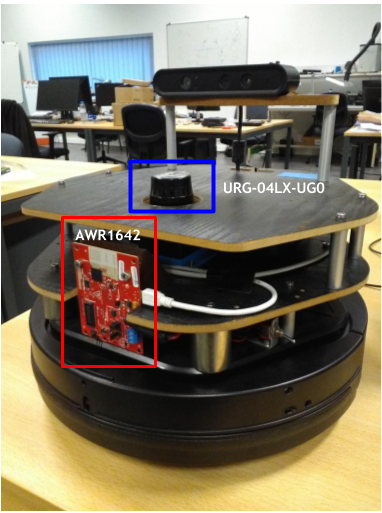
\includegraphics [width=0.4 \textwidth]{imgs/chapter4/turtlebot2.PNG}}
\caption{Modified Turtlebot2 used in this work}
\label{fig::turlebot2M}
\end{figure}

\subsection{Turtlebot2}
TurtleBot 2 (Fig. \ref{fig:t2}) is one of the  most popular low cost personal robots around. It is completely run by open source software which makes it exceptional for research and educational purposes. The robot has been developed by the Korean company Yujin Robotics in collaboration with Willow Garage. Its differential kinematics mobile platform can be used for multiple applications, due to the huge number of available ROS packages. 
%It comes with a kobuki base a processing unit Intel NUC, the 2-D \ac{LiDAR} Hokuyo URG-04LX-UG01 Scanning Laser Rangefinder and finally a Kinect for XBOX 360.

\begin{figure}[ht!] 
\centerline{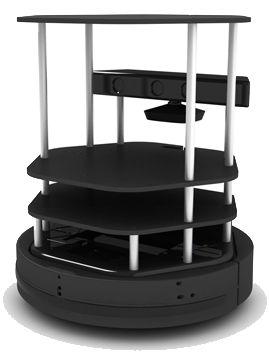
\includegraphics [width=0.3 \textwidth]{imgs/chapter4/turtlebot2.png}}
\caption{Turtlebot 2 platform}
\label{fig:t2}
\end{figure}

When it comes to technical specifications the robots dimension is 354 x 354 x 420 mm as shown in Fig. \ref{fig::t2specs}, its weight is 6.3 Kg with a max payload of 5 Kg which means it is able to attach lots of sensor devices with if needed. Its maximum translational  speed is 0.7 m/s and the maximum rotational speed is 180º/s . It is equipped with a gyroscope with 1 axis(110º/s), an odometer at 52 ticks/encoder and  bumpers on left, right and center among other components. 

\begin{figure}[ht!] 
\centerline{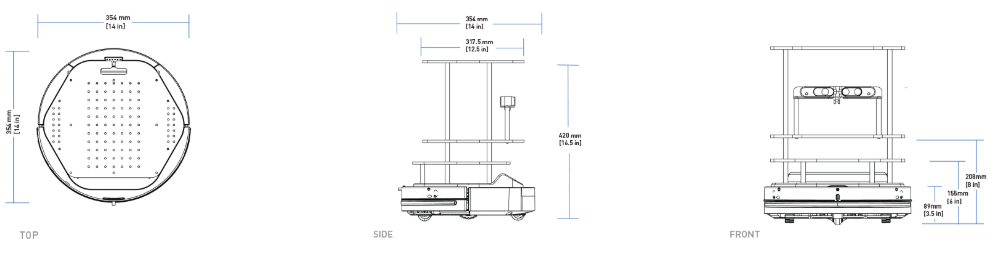
\includegraphics [width=1.0 \textwidth]{imgs/chapter4/tspecs.png}}
\caption{Turtlebot 2 dimension specifications}
\label{fig::t2specs}
\end{figure}


\subsection{FMCW radar}
The radar board chosen for this work is the mmWave \ac{TI} AWR1642BOOST (Fig.\ref{fig:awr}). This is a recently distributed \ac{FMCW} radar appropriate for short range applications. It is an easy-to-use evaluation board for the AWR1642 automotive radar sensor which is connected to the micro-controller unit (MCU) LaunchPad. To develop software it has  on-chip C67x DSP core and low-power ARM Cortex-R4F controllers which include onboard emulation for programming and debugging.
It requires a 5V > 2.5 A supply brick with a 2.1-mm barrel jack to run.
The device supports a wide RF bandwidth of 77-81 GHz that permits good range, velocity  and angle resolution. These last parameters depend on the configuration fed to the device.

\begin{figure}[ht!] 
\centerline{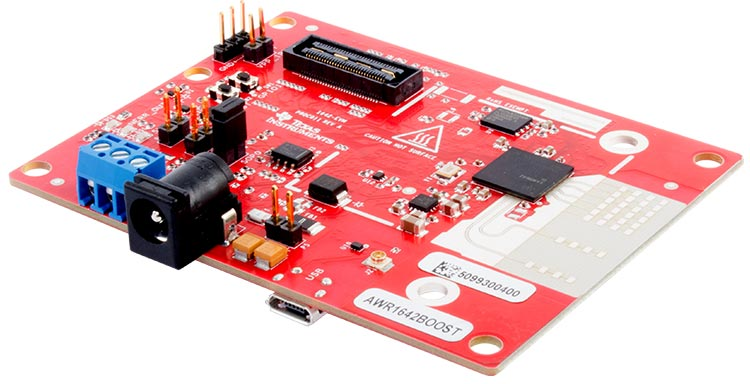
\includegraphics [width=0.5 \textwidth]{imgs/chapter4/awr1642.jpg}}
\caption{Texas Instruments AWR1642BOOST evaluation board}
\label{fig:awr}
\end{figure}


The radiation pattern of the antenna in the horizontal plane (H-plane Phi = 0 degrees) and elevation plane (E-plane Phi= 90 degrees) is shown by Figure \ref{fig:el}.
\begin{figure}[ht!] 
\centerline{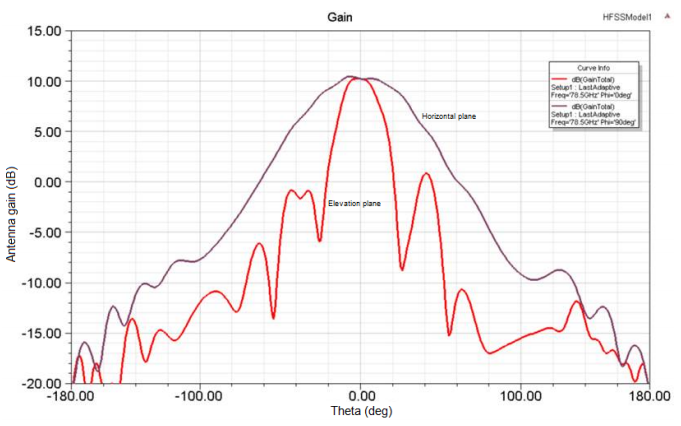
\includegraphics [width=0.9 \textwidth]{imgs/chapter4/elevation.png}}
\caption[Radiation pattern of the antenna]{Radiation pattern of the antenna from \cite{el}}
\label{fig:el}
\end{figure}

\subsection{LiDAR}
Besides the \ac{FMCW} \ac{radar} the Hokuyo URG-04LX-UG01 Scanning Laser Rangefinder (Fig. \ref{fig:lidarP}) is also attached to the platform.

This sensor is an inexpensive 2D-\ac{LiDAR} that is based on phase difference measurement. It retrieves information of the surrounding environment by scanning an area of 240º with 0.36º angular resolution. Its maximum range is about 4 meters and its range resolution is 1mm. Its scan update time is 100ms/scan and its weight is 360 g.  As for the power supply it only needs a 5V DC provided by the USB connection as shown in Figure \ref{fig::lidarS}.



\begin{figure}[ht!]
  \centering
  \begin{subfigure}[t]{0.35\linewidth}
    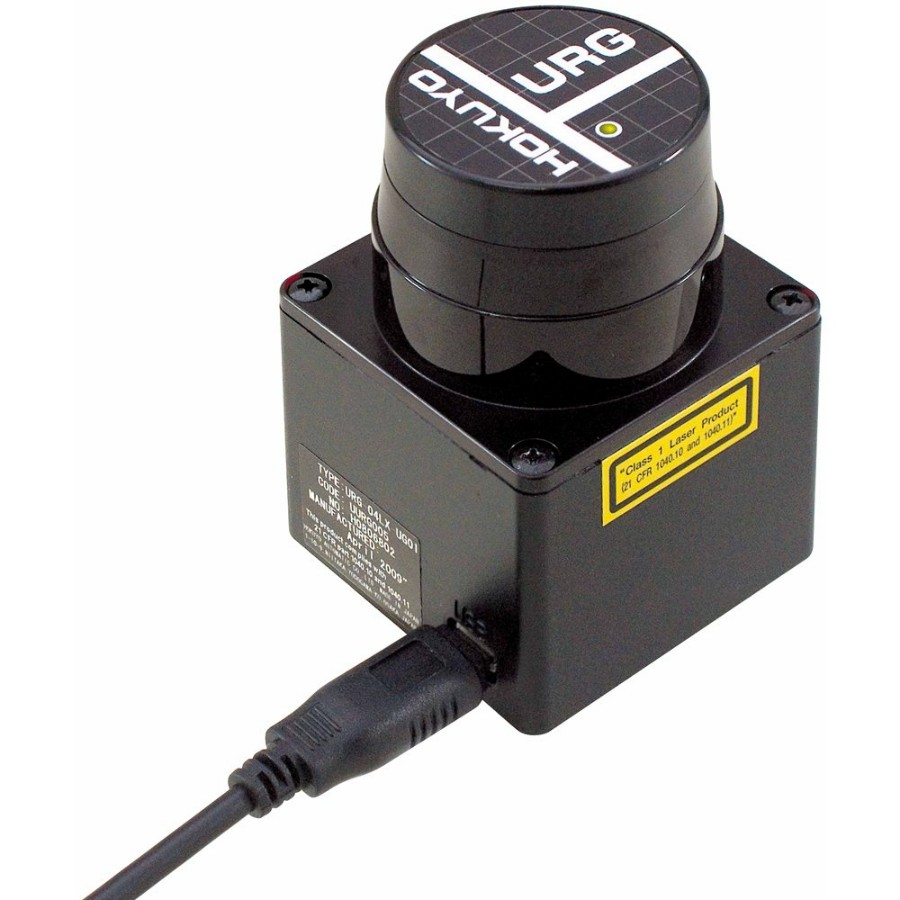
\includegraphics[width=\linewidth]{imgs/chapter4/lidar.jpg}
     \caption{Hokuyo URG-04LX-UG01 Scanning Laser Rangefinder}
     \label{fig:lidarP}
  \end{subfigure}
  \begin{subfigure}[t]{0.55\linewidth}
    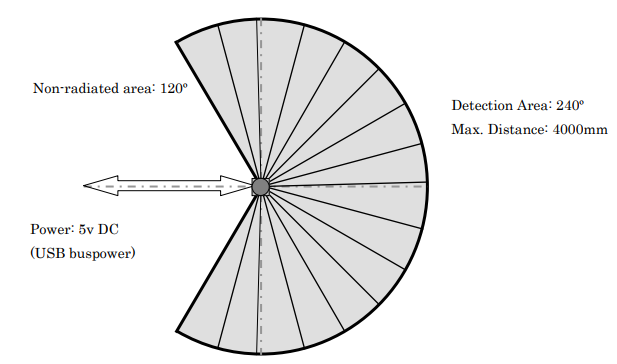
\includegraphics[width=\linewidth]{imgs/chapter4/lidarS.png}
    \caption{Hokuyo URG-04LX-UG01 specifications diagram}
    \label{fig::lidarS}
  \end{subfigure}
  \caption{Hokuyo URG-04LX-UG01 Scanning Laser Rangefinder overview }
  \label{fig:lidar}
\end{figure}


\section{Software}
Figure \ref{fig::softsetup} shows the block diagram describing  the different modules used to have a proper autonomous navigation platform.
\begin{figure}[h] 
\centerline{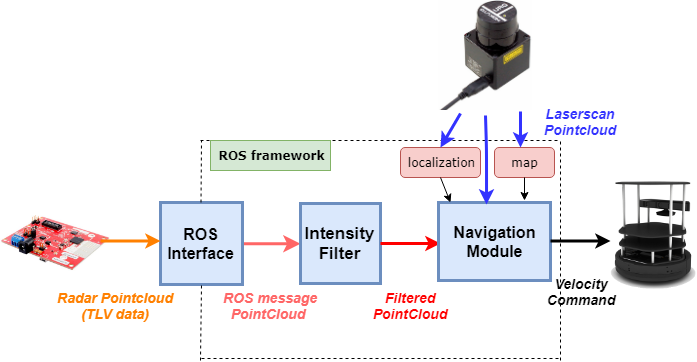
\includegraphics [width=1.0 \textwidth]{imgs/chapter4/bd.png}}
\caption{Block diagram of the software architecture designed for this work}
\label{fig::softsetup}
\end{figure}

First of, a map of the surrounding  environment must first be created.  There are multiple packages for doing this in \ac{ROS}, but in our case we used the package \texttt{gmapping} with 2D-\ac{LiDAR} as input. The robot also needs to be able to localize itself, for that we will use again the 2D-\ac{LiDAR} for input in the package \texttt{amcl}. This will update the localization of the robot taking into account the odometry information and the observable environment. With localization and mapping problem taken care of we now must feed the Navigation Module with obstacle detectors. For that we use the 2D-LiDAR and the radar data as sensor sources.
 However the radar data is not compatible with the \ac{ROS} navigation module. It sends \ac{TLV} data that must be decoded and converted to a \ac{ROS} message format. To do this conversion we have a block called \ac{ROS} Interface. After this is done we encountered false positive obstacles detected by the radar so we added a new module that processes the radar message to combat this issue, we calll it an Intensity Filter. Finally, with this processing done, we feed the Navigation Module with the processed radar data in \ac{ROS} format or/and the 2D-\ac{LiDAR} as obstacle detectors. 
%In order to produce a suitable platform for navigation we need to interconnect various software modules in \ac{ROS}. First a map of the environment is created by the 2-D \ac{LiDAR} using the package \texttt{gmapping}. After that is done we launch the \texttt{amcl} node that will update the localization of the robot taking into account odometry information and the surrounding environment. After that is done we have a robot that is reasonably well localized. Now all we need is to feed some sensor sources to the navigation module that will act as obstacle detectors.

%To do that, first the interface between the radar board TLV data and the ROS point cloud message format is done using the provided radar driver from Texas Instruments.  Then a filter by intensity operation is added to remove false positive detections (this will be explained later). The filtered radar data as well as the \ac{LiDAR} data are fed to the Navigation module as sensor sources.




\subsection{ROS Interface}
In order to use the radar for obstacle detection we must first convert the \ac{TLV} data of the robot to the \ac{ROS} message format.
To do this Texas Instruments provides a \ac{ROS} package that interfaces radar data to the ROS framework \cite{tisetup}. The incoming radar \ac{TLV} data from the radar is decoded in order to create a  \textbf{PointCloud2} type ROS message.
This point cloud follows the detected objects frame described in the mmWave demo data structure \cite{mmdata} represented in Fig. \ref{fig:demodata}.
\begin{figure}[!htb]
    \centering
    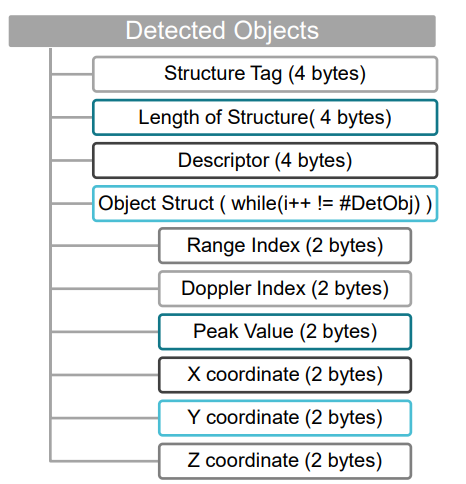
\includegraphics[scale=0.6]{imgs/chapter4/demodata.png}
    \caption[Part of the mmwave demo packet]{Part of the mmwave demo packet containing object detection information. This fields will be used to construct the ROS PointCloud2 \cite{mmdata}.}
    \label{fig:demodata}
\end{figure}
Each point has 6 fields:
\begin{itemize}
\item \textbf{x (m)} - position x of the detected  object in the frame of the radar.
\item \textbf{y (m)} - position y.
\item \textbf{z (m)} - position z (for 2D devices this is equal to zero).
\item \textbf{range (m)} - range of the object relative to the radar frame.
\item \textbf{doppler (m/s)} - radial velocity of the object relative to the radar frame.
\item \textbf{intensity} - power of the received signal corresponding to that object.
\end{itemize}

The characteristics of the \ac{radar} data, such as publishing rate, range resolution, maximum range, velocity, resolution and maximum velocity depends on the chirp profile configuration file loaded in the \ac{radar}.
The easiest way to create a chirp configuration file is using the mmWave Demo Visualizer. With it you can auto generate a configuration file given a set of specifications.
Another way of doing this is manually. This however requires the understanding of the radar operating principle and the configuration commands.




%Describe PCL

\subsection{Visualization of the radar point cloud}
Plotting the points in the XYZ space is not enough to fully visualize the radar data sent since each point also gives velocity and intensity information. We can better visualize it by using markers such as arrows or text in rviz.
Figure \ref{fig:dopplermarker} displays the radial velocity of each point with an arrow. The width of the arrow indicates how fast in the direction  of the radar the object is going. Figure \ref{fig:intensitymarker} shows the intensity values of each object in text. This type of visualization will be useful when we want to filter the cloud.


\begin{figure}[ht!]
  \centering
  \begin{subfigure}[b]{0.49\linewidth}
    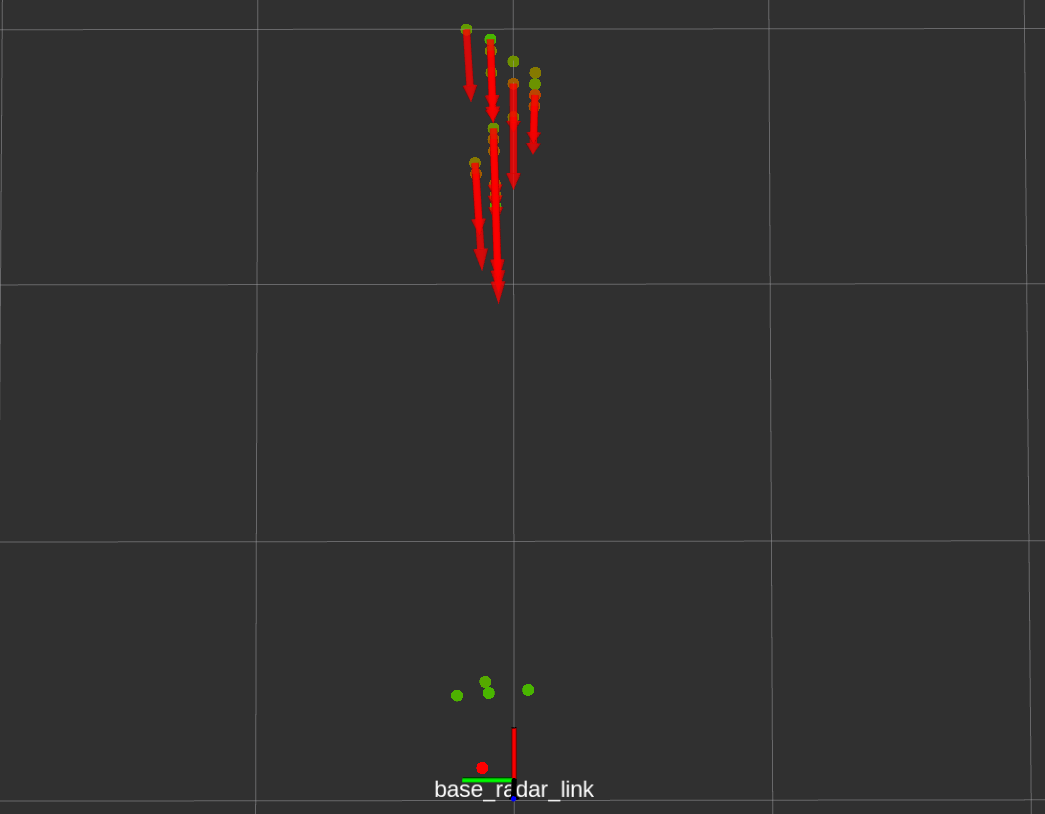
\includegraphics[width=\linewidth]{imgs/chapter4/dopplermarker.png}
     \caption{Arrow markers displaying the points radial velocity}
     \label{fig:dopplermarker}
  \end{subfigure}
  \begin{subfigure}[b]{0.44\linewidth}
    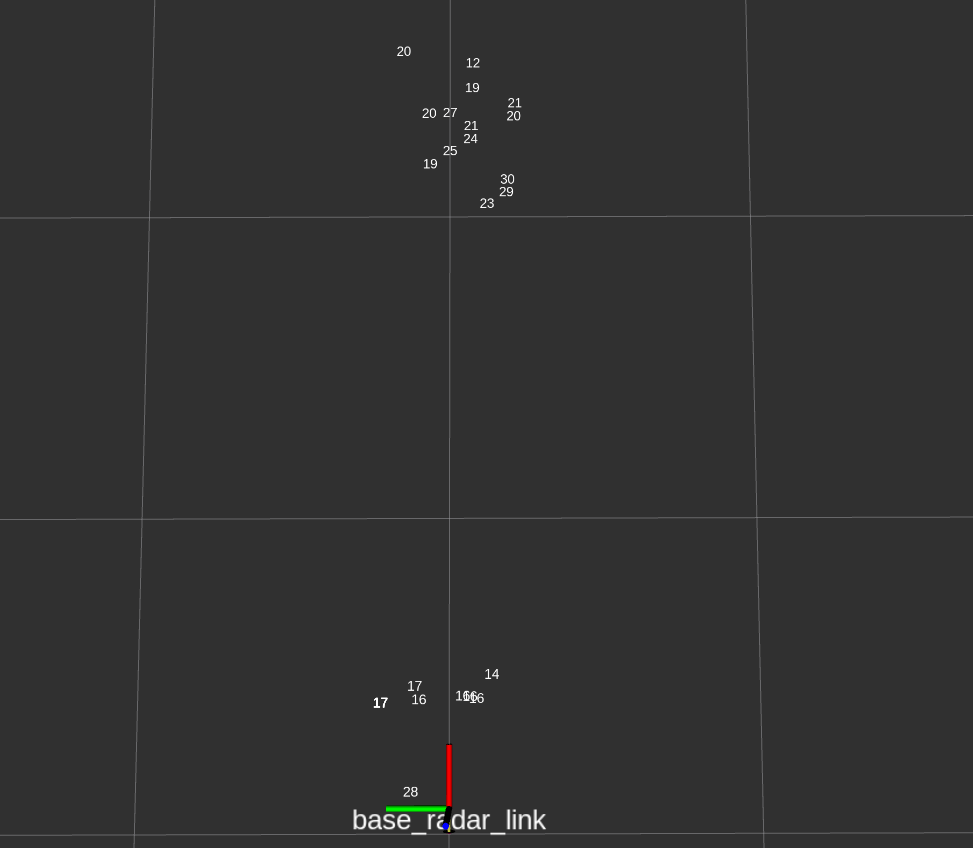
\includegraphics[width=\linewidth]{imgs/chapter4/intensitymarker.png}
    \caption{Text markers displaying the points intensity values}
    \label{fig:intensitymarker}
  \end{subfigure}
  \caption{Visualization markers displaying radar data information}
  \label{fig:vismark}
\end{figure}


\subsection{Intensity Filter}
Since we are dealing with point clouds coming from the \ac{FMCW} \ac{radar} and the 2-D\ac{LiDAR} than we need some type of ways to handle and manipulate them. For that the open source libraries called \ac{PCL} is the more indicated place to process and manipulate this type of information. A pointcloud is a collection of multi-dimensional points and is commonly used to represent three-dimensional data \cite{pcl}. These points are often just designed to locate points in x,y,z but more dimensions can be added as is for the FMCW radar which has 6 dimensions. \ac{PCL} provides open source, state of the art library modules that enables  filtering, feature estimation, surface reconstruction, registration, model fitting and segmentation. 

%and \textbf{euclidean clustering} to identify groups of points that belong to the same object.
In the point cloud there may be some points that have undesirable characteristics, such as points with low intensity  that lead to false detections or outside of the radar operating range. To remove these points we use \textbf{passthrough filters} that specify the range of values a given field can have in order for a point to be kept in the point cloud. 

For example, if we are only interested in obstacles that are moving between 0.5 m/s and 1.0 m/s (radial velocity), this can be done by using a passthrough filter on the doppler channel.
Figure \ref{fig:filters} shows an example where we delete detections close to the radar by filtering the point cloud by intensity. In this work we will use an intensity filter of 16, which means all target points that have an intensity bellow that will be filtered out due to having a low \ac{SNR}


\begin{figure}[ht!] 
    \begin{minipage}[b]{.49\linewidth}
        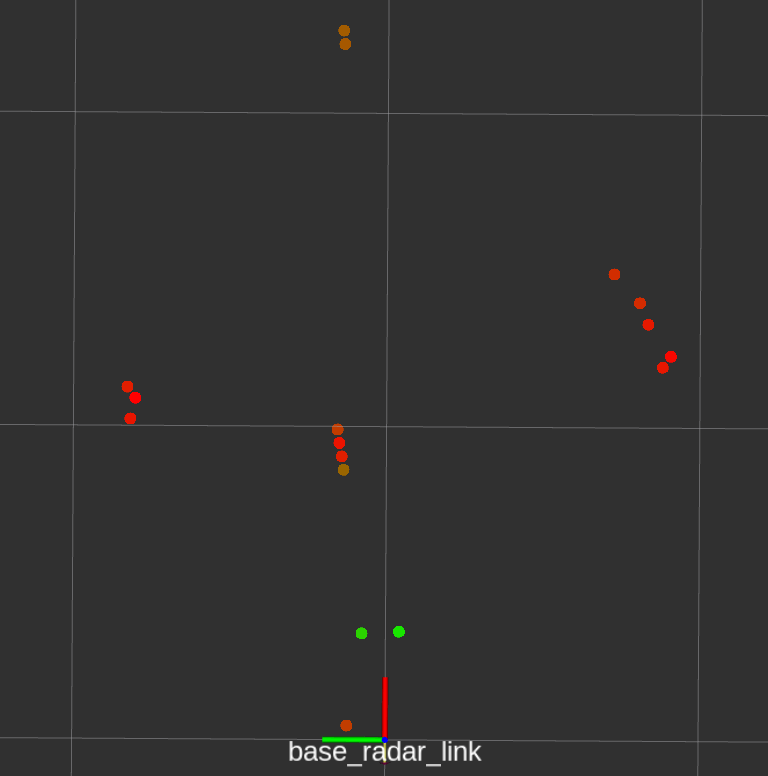
\includegraphics[height=5cm,width=\linewidth]{imgs/chapter4/notfilt.png}
        \subcaption{Non filtered pointcloud}
        \label{fig:nonfilt}
    \end{minipage}
    \begin{minipage}[b]{.49\linewidth}
        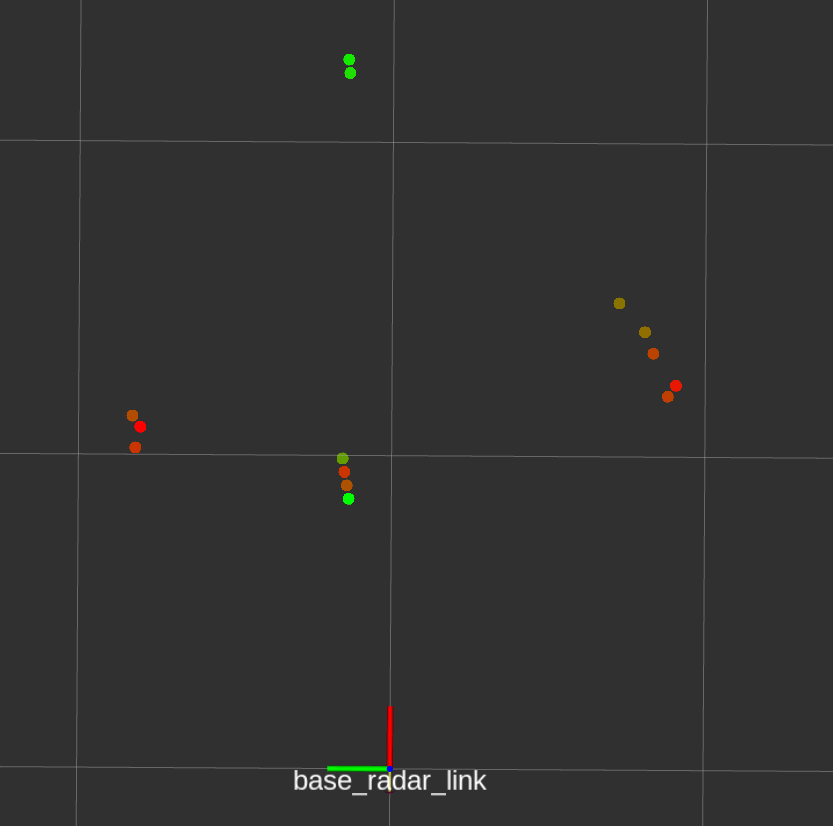
\includegraphics[height=5cm,width=\linewidth]{imgs/chapter4/filt.png}
        \subcaption{Filtered pointcloud by intensity}
        \label{fig:filt}
    \end{minipage}
    \caption{Example of filtering the pointcloud}
    \label{fig:filters}
\end{figure}
\subsection{Navigation Module}
The navigation module first needs a map in order to have a global frame as reference. After that we need to localize the robot in said map, for that we use the \ac{AMCL} node. Finally we need range sensors that detect obstacles.
With the processed \ac{radar} data we can now feed it to our navigation system. We can either feed the \ac{LiDAR} or/and \ac{FMCW} \ac{radar} as obstacle detectors. 
The navigation module will then use all this information to compute the velocity command  that will make the turtlebot2 move.


\section{Summary}
In this chapter we overviewed the technical specifications of each hardware component in the navigation platform that will be used on in this work. We also overview what software and how it is interconnected  to properly setting up the turtlebot2 robot for indoor navigation.


%The software used in this project is divided in a few stages. First the interface between the radar board TLV data and the ROS point cloud message format is done using the provided radar driver from Texas Instruments.  Then a filter by intensity operation is added to remove false detections (this will be explained later). The filtered radar data as well as the \ac{LiDAR} data are fed to the ROS Navigation Stack as sensor sources. In terms of mapping a f